\documentclass[twocolumn]{article}
\usepackage[utf8]{inputenc}
\usepackage{multicol}
\usepackage[english]{babel}
\usepackage{blindtext}
\usepackage{authblk}
\usepackage{graphicx}
\usepackage{amsmath}
\usepackage{hyperref}
\newtheorem{theorem}{Theorem}[section]
\newtheorem{corollary}{Corollary}[theorem]
\newtheorem{lemma}[theorem]{Lemma}

\title{All-pairs  suffix/prefix  in  optimal  time  using  Aho-Corasick space}
\author[a]{Grigorios Loukides}
\author[b, c, *]{Solon  P. Pissis}
\affil[a]{Department of Informatics, King’s College London, London, UK}
\affil[b]{CWI, Amsterdam, the Netherlands}
\affil[c]{Vrije Universiteit, Amsterdam, the Netherlands}

\date{}

\begin{document}
\maketitle



\section*{Abstract}

The all-pairs suffix/prefix (APSP) problem is a classic problem in computer science with many applications in bioinformatics. Given a set $\{ S_1, \ldots , S_k \}$ of $k$ strings of total length $n$,  we  are  asked  to  find,  for  each  string  $S_i,  i \in [ 1, k]$,  its  longest  suffix  that  is  a  prefix of string  $S_j$, for all  $j \neq i,  j \in [ 1, k]$.

\section*{Keywords}
\begin{itemize}
    \item Algorithms
    \item Data Structures
    \item String algorithms
    \item Aho-Corasick Machine
\end{itemize}

\section{Introduction}

Given a set $R = \{ S1, . . . ,  Sk \}$ of $k$ strings of total 
length $n$, the APSP problem asks us to find, for each string 
$S_i, i \in [1, k]$, its longest suffix that is a prefix of string  $S_j$, 
for  all  $j \neq i,  j \in [1, k]$. \\

\textit{Other related work.} In  addition  to  $l$-APSP that  is  formulated  in  this  paper,  there  are  two  other  versions  of  APSP 
that  have  been  studied  in  the  literature. \\

\textit{Paper organization.} Section 2 presents some preliminaries 
and our main result. Section 3 presents the algorithm we 
develop. Section 4 concludes the paper.

\section{Preliminaries and main result}

An \textit{alphabet} $\Sigma$ is a finite nonempty set whose elements 
are  called  \textit{letters}.  A  string $S = S[1 . . m]$ is  a  sequence  of \textit{length} $|S| = m$ over $\Sigma$.  The  \textit{empty string} $\epsilon$ is  the  string  of 
length  0. The \textit{} of two strings  $S$ and  $T$ is the string composed of the letters of  $S$ followed by the letters 
of  $T$ ;  it  is  denoted  by  $S \dot T$ or  simply  by  $ST$.  For  $1 \leq i \leq
j \leq m$,  $S[i]$ denotes  the  $i$th  letter  of  $S$,  and  the  fragment 
$S[i . .  j]$ denotes  an  occurrence of  the  underlying  substring
$P = S[i] · · · S[j]$. We say that  P \textit{occurs} at (starting) \textit{position}
$i$ in  $S$. A fragment  $S[i . .  j]$ is a \textit{suffix} of  $S$ if  $j = m$, and it is 
a prefix of  $S$ if $i = 1$. A substring of  $S$ is called proper if it 
is not equal to  $S$. Given two strings  $S$ and $T$ , a suffix/prefix 
overlap of  $S$ and  $T$ is  a  suffix  $U$ of  $S$ that  is  a  prefix  of 
$T$ ; when $U$ is the longest such suffix, then $U$ is called the 
maximal suffix/prefix overlap of  $S$ and $T$ .

\pagebreak

\begin{figure}[!htb]
    \centering
    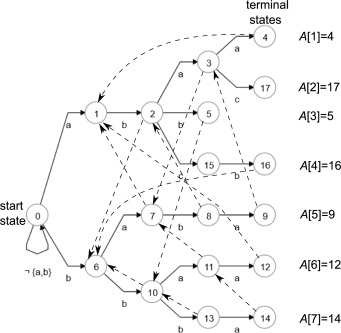
\includegraphics{Fig. 1.jpg}
    \caption{The AC machine over $R = \{ abaa, abac, abb, abcb, baba, bbaa,
bbba \}$. Solid arrows correspond to goto transitions and dashed arrows to failure transitions. The lexicographic ranks of the strings in $R$ are the indices of array $A$}
    \label{fig:my_label}
\end{figure}

\begin{lemma}
\textit{(Aho-Corasick lemma [1]). Let state s correspond to 
string U and  state t correspond to string V in  the AC machine of 
a set R of  strings. Then, we have that  f (s) = t if  and only if V is  
the longest proper suffix of U that  is also a prefix of some string 
in R}
\end{lemma}

\section{The Algorithm}

\subsection{Reducing the $l$-APSP problem to the ULIT problem}

Given a collection  $I = \{ [ i1, j1]d1 , . . . ,  [ir, jr]dr \} $
of $r$ labeled intervals, we define the union of $I$ as the set

$$U(I) = \{ e_d : e \in [i,j]_d \in I \,\, \textbf{and} \,\, \nexists e \in [i', j']_{d'} \in I : d' > d \}$$

\noskip \textbf{Definition 1} (Failure transition tree (FTtree)). Given  a  set  $R$
of strings, the failure transition tree (FTtree, for short) of  $R$
is the rooted tree induced by the set of (reversed) failure 
transitions of the AC machine of  $R$.\\

We prove the following lemma.

\begin{lemma}
\textbf{Lemma 2.} \textit{Any instance of the -APSP problem can be reduced 
to some instance of the ULIT problem in O(n) time.}
\end{lemma}

\begin{figure}
    \centering
    \includegraphics{Fig. 2.jpg}
    \caption{FTtree $T_1$ for $l$ = 1. The output set per leaf node is in a squared box}
    \label{fig:my_label2}
\end{figure}

\begin{figure}
    \centering
    \includegraphics{Fig. 3.jpg}
    \caption{FTtree $T_2$ for $l$ = 2. The output set per leaf node is in a squared box}
    \label{fig:my_label3}
\end{figure}

\subsection{Solving the ULIT Problem}


A branching node of T is a non-root node with at least 
two  children.  A  branchless subpath is  an  upward  maximal 
path  of  nodes  starting  from  a  branching  node  or  a  leaf 
node and ending at the node right before a branching node

\begin{table}[!htb]
\begin{tabular}{lll}
\hline
\begin{tabular}[c]{@{}l@{}}Branchless \\ Subpaths\end{tabular} & \begin{tabular}[c]{@{}l@{}}Sorted\\ Tuples\end{tabular}         & \begin{tabular}[c]{@{}l@{}}Compact\\ Represen-\\ tation\\ of the\\ Union\end{tabular} \\ \hline
1                         & (1,1,4,1)                                                       & $\{{[}1,4{]}_1\}$                                                                      \\
4           & (4,1,1,4)                                                       & $\{{[}1,1{]}_4\}$                                                                      \\
5$\rightarrow$10                                                           & \begin{tabular}[c]{@{}l@{}}(5,3,3,3)\\ (5,6,7,2)\end{tabular}   & $\{{[}3,3{]}_3$, ${[}6,7{]}_2\}$                                                        \\
6                & (6,5,7,1)                                                       & $\{{[}5,7{]}_1\}$                                                                      \\
7                & (7,5,5,2)                                                       & $\{{[}5,5{]}_2\}$                                                                      \\
9$\rightarrow$3                                                            & \begin{tabular}[c]{@{}l@{}}(9,1,2,3)\\ (9,5,5,4)\end{tabular}   & \{{[}1,2{]}\_3,{[}5,5{]}\_4\}                                                         \\
12                            & (12,6,6,4)                                                    & $\{{[}6,6{]}_4\}$                                                                      \\
14$\rightarrow$11                                                          & \begin{tabular}[c]{@{}l@{}}(14,6,6,3)\\ (14,7,7,4)\end{tabular} & \{{[}6,6{]}\_3,{[}7,7{]}\_4\}                                                         \\
16               & (16,4,4,4)            & $\{\{4,4{]}_4\}$                                                                       \\
17                      & (17,2,2,4)                                                      & $\{{[}2,2{]}_4\}$                                                                      \\ \hline
\end{tabular}
\end{table}

\begin{figure}[!htb]
    \centering
    \includegraphics[scale=0.5]{Fig. 4.jpg}
    \caption{Step 3 using the FTtree in Fig. 2. At each branching node, we store the resulting union. At each leaf node, we store the output in a squared box.}
    \label{fig:my_label}
\end{figure}

(or the root node if no branching node exists). For exam-
ple, the branchless subpaths in Fig. 2 are shown in Table 1. 
The algorithm for solving the ULIT problem works as fol-
lows:

\begin{enumerate}
    \item Decompose $T_l$ into a set of branchless subpaths. Using 
a  DFS  traversal  on  $T_l$,  for  each  node  decorated  with 
[i, j]d of every branchless subpath starting with node 
u, construct a tuple $(u, i, j, d)$.

\item Sort all tuples constructed in Step 1 together. For each 
branchless  subpath,  take  the  compact  representation 
of  the  union  of  its  set  of  labeled  intervals,  which  are 
now sorted. Inspect Table 1.

\item Visit  the  branching and  leaf nodes using  a  BFS  traver-
sal on  $T_l$. From node u to node  v, such that  v is the 
child  of  u,  take  the  union  of  the  two  sets  of  labeled 
intervals (one from u and one from v), and update the 
union associated with v. At the leaf nodes we have the 
output sets. Inspect Fig. 4.
\end{enumerate}

The  following  lemma  together  with  Lemma 2 implies
Theorem 1.\\

\begin{lemma}
\textbf{Lemma  3.} The  ULIT  problem  can  be  solved  in  $\mathcal{O(N)} +
|\textit{OUTPUTK} |)$ time using $O(N)$ space.\\
\end{lemma}


\section{Final Remarks}

\hskip2em All existing optimal algorithms for APSP rely on sorting 
the  suffixes  of  all  strings  in  R.

\section*{Declaration of competing interest}

\hskip2em The authors declare that they have no known competing financial interests or personal relationships that could have  appeared  to  influence  the  work  reported  in  this  paper.

\section*{Acknowledgements}

\hskip2em The  authors  would  like  to  thank  Anne  Luesink  (Vrije 
Universiteit)  for  implementing  the  algorithm  underlying 
Theorem 1.  The  source  code  is  freely  available  at  \href{https://github.com/ALuesink/APSP_algorithm}{wat}

\section*{References}

\end{document}